\begin{experiment}{Three possible voting aproaches.}{\small \sffamily\textbf{Description}

We are testing limit on range 1---35 using heart dataset, analyzing:

\begin{itemize}
\tightlist
	\item \texttt{LON} --- \emph{Same weights for all \emph{exposers}}, an ensemble, using \textbf{random} approach, grain \emph{30}, radius \emph{0.1}, dimensions \emph{[2]}, using \textbf{lone participation}.
	\item \texttt{TH1} --- \emph{One weight per \emph{exposer}}, an ensemble, using \textbf{random} approach, grain \emph{30}, radius \emph{0.1}, dimensions \emph{[2]}, using \textbf{single measure per exposer}.
	\item \texttt{TH2} --- \emph{One weight per \emph{class}}, an ensemble, using \textbf{random} approach, grain \emph{30}, radius \emph{0.1}, dimensions \emph{[2]}, using \textbf{single measure per class}.

\end{itemize}


\textbf{Results}

\centering
	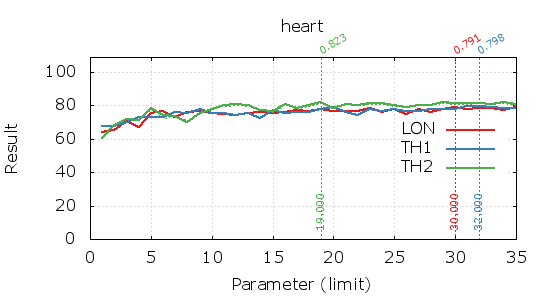
\includegraphics[width=.75\textwidth]{plots/experiment_5_heart.png}
	\captionof{figure}{Three possible voting aproaches.}
	\label{fig:experiment_5}
}\end{experiment}